\documentclass[12pt]{report}

\usepackage{commands}


\begin{document}

\large

\begin{center}
 Math 586 Homework 5\\
 Due June 2\\
 By Marvyn Bailly (Github: MarvynB)\\
\end{center}

\normalsize

\hrule


%---------------%
%---Problem 1---%
%---------------%

%--status--$

\begin{problem}
    Consider solving
    \begin{align*}
        \begin{cases} u_t + u_{xxx} = 0, \quad -1 < x < 1\\
            u(x,0) = \eta(x),\\
            u(-1,t) = u(1,t),\\
      u_x(-1,t) = u_x(1,t),\\
      u_{xx}(-1,t) = u_{xx}(1,t).\end{cases}
    \end{align*}
    This is the linear KdV (Airy) equation with periodic boundary conditions.
    \begin{itemize}
        \item Use a second-order accurate centered difference and the trapezoid method as a time-stepper. Can you see dispersive quantization? Use $\eta(x) = 1$ if $-1/2 < x < 1/2$ and $\eta(x) =0$ otherwise.
        \item Prove that the method is Lax-Richtmyer stable.  Discuss whether or not it is convergent with this initial condition.
    \end{itemize}
\end{problem}

\begin{solution}

    \noindent
    Consider the Airy equation with periodic boundary conditions given by
    \begin{align*}
        \begin{cases} 
            u_t + u_{xxx} = 0, \quad -1 < x < 1\\
            u(x,0) = \eta(x),\\
            u(-1,t) = u(1,t),\\
            u_x(-1,t) = u_x(1,t),\\
            u_{xx}(-1,t) = u_{xx}(1,t).
        \end{cases}
    \end{align*}
    \begin{enumerate}
        \item [(a)]
        We first wish to solve the problem using a second-order accurate centered difference and the trapezoid method as a time stepper. We begin by discretizing in space using a centered finite difference of the form
        \[
            U_j'(t) = -\paren{\frac{-U_{j-2}(t) + 2U_{j-1}(t) - 2U_{j+1}(t) + U_{j+2}(t)}{2h^3}}[U_j].
        \] 
        Then applying the periodic boundary conditions we have that
        \begin{align*}
            U_0 &= U_{m+1}\\
            U_{-1} &= U_{m}\\
            U_{-2} &= U_{m-1}.
        \end{align*}
        Then at $j=0$ we have
        \[
            U_0' = \frac{-U_{-2} + 2U_{-1} - 2U_{1} + U_{2}}{2h^3} = \frac{-U_{m-1} + 2U_{m} - 2U_{1} + U_{2}}{2h^3},
        \]
        and at $j=1$ we have
        \[
            U_1' = \frac{-U_{-1} + 2U_{0} - 2U_{2} + U_{3}}{2h^3} = \frac{-U_{m} + 2U_{m+1} - 2U_{2} + U_{3}}{2h^3},
        \]
        and at $j=2$ we have
        \[
            U_2' = \frac{-U_{0} + 2U_{1} - 2U_{3} + U_{4}}{2h^3} = \frac{-U_{m+1} + 2U_{1} - 2U_{3} + U_{4}}{2h^3},
        \]
        and continuing this process we find 
        \[
            [U'_j] = -\frac{1}{2h^3}D_3[U_j], 
        \]
        where
        \[
            D_3 = \begin{bmatrix}
            0 & -2 & 1 &&& -1 & 2\\
            2 & 0 & -2 & 1 &&& -1 \\
            -1 & 2 & 0 & -2 & 1 \\
            & \ddots & \ddots & \ddots & \ddots & \ddots \\
            && -1 & 2 & 0 & -2 & 1 \\
            1 &&& -1 & 2 & 0 & -2 \\
            -2 & 1 &&& -1 & 2 & 0
            \end{bmatrix}
        \]
        Then applying the trapezoid method to time step yields 
        \[
            \paren{I + \frac{k}{4h^3}D_3}[U^{n+1}_j] = \paren{I-\frac{k}{4h^3}D_3}[U^n_j].    
        \]
        We implement this method in Julia as follows:
        \begin{python}
function solve_airy(m,inti,stop)
    L = 1
    h = 2/(1+m)
    k = 0.01
    xs = -1:h:1-h
    h = L*h
    xs = L*xs

    D3 = diagm(1 => fill(-2,m), -1 => fill(2,m), -2 => fill(-1,m-1), 2 => fill(1,m-1)) |> sparse
    D3[1,m] = -1
    D3[1,m+1] = 2
    D3[2,m+1] = -1
    D3[m+1,1] = -2
    D3[m+1,2] = 1
    D3[m,1] = 1
    
    U = inti.(xs)
    for t=k:k:stop
        U =  (I + k/(4*h^3)*D3) \ ((I-k/(4*h^3)*D3)*U)
    end
    return xs, U
end
        \end{python}
        Then using $h = 0.004$ and $k=0.01$ and plotting the solution at rational numbers of the period length such as $t \in [0.25,0.50,0.75,1.0]$ we get plots seen in Figure \ref{fig1}. Recalling that the initial condition is a step function, we see no signs of dispersive quantization in this system since the solution does not appear to be a composition of step functions as we would expect when dispersive quantization is present. 

        \begin{figure}[H]
            \begin{subfigure}[b]{0.45\linewidth}
                \centering
                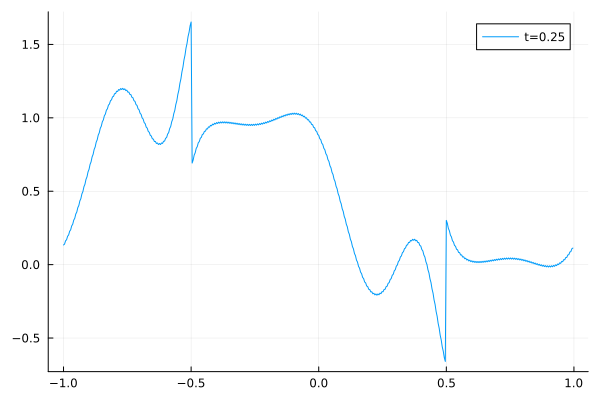
\includegraphics[width=\linewidth]{images/1-1.png}
                \caption{Solution at $t=0.25$.}
                \label{fig1:a}
                \vspace{4ex}
            \end{subfigure}%%
            \begin{subfigure}[b]{0.45\linewidth}
                \centering
                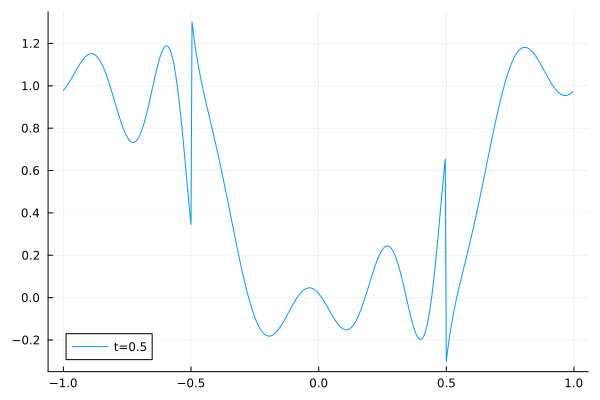
\includegraphics[width=\linewidth]{images/1-2.png}
                \caption{Solution at $t=0.50$.}
                \label{fig1:b}
                \vspace{4ex}
            \end{subfigure}
            \begin{subfigure}[b]{0.45\linewidth}
                \centering
                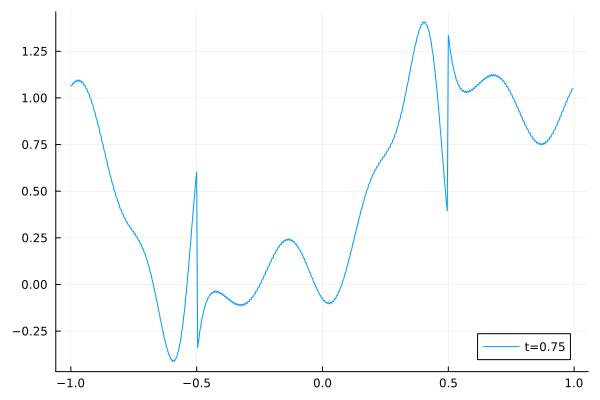
\includegraphics[width=\linewidth]{images/1-3.png}
                \caption{Solution at $t=0.75$.}
                \label{fig1:c}
                \vspace{4ex}
            \end{subfigure}%%
            \begin{subfigure}[b]{0.45\linewidth}
                \centering
                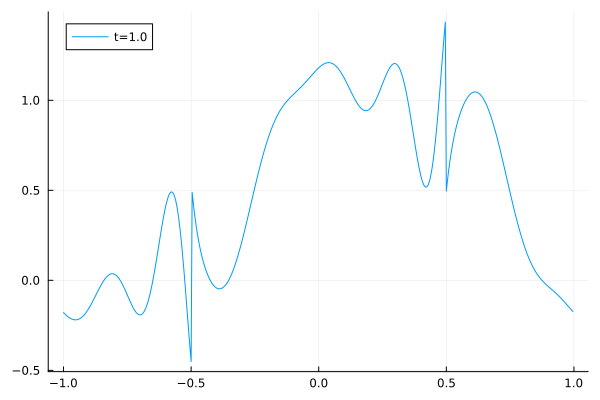
\includegraphics[width=\linewidth]{images/1-4.png}
                \caption{Solution at $t=1.0$.}
                \label{fig1:d}
                \vspace{4ex}
            \end{subfigure}
            \caption{Solutions at $t=[0.25,0.50,0.75,1.0]$ to the linear KdV equation using a second-order accurate method.}
            \label{fig1}
        \end{figure}    


        \item [(b)]
        To apply Lax-Richtmyer stability analysis, we require $(I+\frac{k}{4h^3}D_3)$ to be invertible. Since $D_3$ is scew-symmetric, so is $\frac{k}{4h^3}D_3$. We know that skew-symmetric matrices have purely imaginary eigenvalues and thus we know that $I + {4h^3}D_3$ must have nonzero eigenvalues and thus is invertible. So we now consider 
        \[
            [U_J^{n+1}] = \paren{I +\frac{k}{4h^3}D_3}^{-1}\paren{I - \frac{k}{4h^3}D_3}[U_j^n] = B[U_j^n],
        \]
        and for Lax-Richtmyer stability we require the eigenvalues of $B$ to be less than or equal to $1$ with strict inequality for repeated eigenvalues. Now letting $\lambda = ai$ be an arbitrary eigenvalue $\frac{k}{4h^3}D_3$ and noting that the eigenvalues of $I$ are $1$, then
        \begin{align*}
            |\text{eval}(B)|=|(1 + \lambda)^{-1}(1 - \lambda)| = |(1+ai)^{-1}(1-ai)| = |1+ai|^{-1}|1-ai| = 1.
        \end{align*} 
        Next, we will show that the eigenvalues of $D_3$ are unique. Since $D_3$ encodes a periodic operator then we look for eigenvectors that come from period grid functions of the general form
        %j is my position and l is my eval%
        \[
            [V_j^{(l)}] = [e^{2\pi i j l h}], ~~j=0,1,2,\dots,m.
        \]
        We then compute
        \begin{align*}
            D_3[V_j^{(l)}] &= \begin{bmatrix}
                0 & -2 & 1 &&& -1 & 2\\
                2 & 0 & -2 & 1 &&& -1 \\
                -1 & 2 & 0 & -2 & 1 \\
                & \ddots & \ddots & \ddots & \ddots & \ddots \\
                && -1 & 2 & 0 & -2 & 1 \\
                1 &&& -1 & 2 & 0 & -2 \\
                -2 & 1 &&& -1 & 2 & 0
                \end{bmatrix}[V_j^{(l)}]\\
                &=\begin{bmatrix}
                    -2V_1^{(l)} + V_2^{(l)} - V_{{m-1}}^{(l)} + 2V_m^{(l)}\\
                    2V_{0}^{(l)} - 2V_2^{(l)} + V_{{3}}^{(l)} - V_{m}^{(l)}\\
                    \vdots\\
                    -V^{(l)}_{j-2} + 2V^{(l)}_{j-1} - 2V^{(l)}_{j+1} + V^{(l)}_{j+2}\\
                    \vdots\\
                    V_1^{(l)} - V_{m-3}^{(l)} + 2V_{m-2}^{(l)} - 2V_{m}^{(l)}\\
                    -2V_1^{(l)} + V_{2}^{(l)} - V_{m-2}^{(l)} + 2 V_{m-1}^{(l)}
                \end{bmatrix}\\ 
                &=\begin{bmatrix}
                    -2e^{2\pi i l h} + e^{2\pi i 2 l h} - e^{2\pi i (m-1) l h} + 2e^{2\pi i m l h}\\
                    2e^{2\pi i (0) l h} - 2e^{2\pi i 2 l h} + e^{2\pi i 3 l h} - e^{2\pi i m l h}\\
                    \vdots\\
                    -e^{2\pi i (j-2) l h} + 2e^{2\pi i (j-1) l h} - 2e^{2\pi i (j+1) l h} + e^{2\pi i (j+2) l h}\\
                    \vdots\\
                    e^{2\pi i l h} - e^{2\pi i l (m-3) h} + 2e^{2\pi i l (m-2) h} - 2e^{2\pi i l m h}\\
                    -2e^{2\pi i  l h} + e^{2\pi i 2 l h} - e^{2\pi i (m-2) l h} + 2 e^{2\pi i (m-1) l h}
                \end{bmatrix}\\
                &=\begin{bmatrix}
                    e^{2\pi i(0)lh}\paren{2e^{2\pi i (-1) l h}-2e^{2\pi i (1) l h} + e^{2\pi i (2) l h} - e^{2\pi i (-2) l h}}\\
                    e^{2\pi i(1)lh}\paren{2e^{2\pi i (-1) l h} - 2e^{2\pi i (1) l h} + e^{2\pi i (2) l h} - e^{2\pi i (-2) l h}}\\
                    \vdots\\
                    e^{2\pi i(j)lh}\paren{2e^{2\pi i (-1) l h} - 2e^{2\pi i (1) l h} + e^{2\pi i (2) l h}-e^{2\pi i (-2) l h}}\\
                    \vdots\\
                    e^{2\pi i (m-1)}\paren{2e^{2\pi i l (-1) h} - 2e^{2\pi i l (1) h} +e^{2\pi i (2) l h} - e^{2\pi i l (-2) h}}\\
                    e^{2\pi i (m)}\paren{2 e^{2\pi i (-1) l h}-2e^{2\pi i (1) l h} + e^{2\pi i (2) l h} - e^{2\pi i (-2) l h}}
                \end{bmatrix}\\
                &= (4i\sin(-2\pi l h) + 2i\sin(4\pi lh))[V_j^{(l)}].
        \end{align*}
        Since $h = \frac{2}{m+1}$, the eigenvalues of $D_3$ are unique. Therefore $B$ has unique eigenvalues satisfiying the Lax-Richtmyer stability condition. For the given initial condition, the method is not convergent since it is not consistent. We know that the method is not consistent from the part a were we did not observe dispersive quantization. From class, we expect this method to have quantizations and thus the method is not consistent.  
    \end{enumerate}

\end{solution}

%----------------------------------------------------------------------------------------------------%
%\vskip 20pt
\newpage

%---------------%
%---Problem 1---%
%---------------%

%--status--$

\begin{problem}
    Consider solving
    \begin{align*}
        \begin{cases} u_t + 3 (u^2)_x + u_{xxx} = 0, \quad -L < x < L,\\
            u(x,0) = \eta(x),\\
            u(-L,t) = u(L,t),\\
            u_x(-L,t) = u_x(L,t),\\
            u_{xx}(-L,t) = u_{xx}(L,t).\end{cases}
        \end{align*}
        This is the KdV equation with periodic boundary conditions.
        \begin{itemize}
            \item Use a second-order accurate centered difference and the trapezoid method as a time-stepper to solve this problem with
            \begin{align*}
                \eta(x) = 4 \mathrm{sech}(x)^2, \quad L = 10.
            \end{align*}
      Note that you will need to implement Newton's method for this and use it at each time step.
    \item You need not prove this, give some rationale as to why you might hope this method is Lax-Richtmyer stable.  
\end{itemize}
\end{problem}

\begin{solution}

    \noindent
    Consider the KdV equation with periodic boundary conditions given by
    \begin{align*}
        \begin{cases} u_t + 3 (u^2)_x + u_{xxx} = 0, \quad -L < x < L,\\
            u(x,0) = \eta(x),\\
            u(-L,t) = u(L,t),\\
            u_x(-L,t) = u_x(L,t),\\
        u_{xx}(-L,t) = u_{xx}(L,t).\end{cases}
    \end{align*}
    \begin{enumerate}
        \item [(a)]
        Consider the initial condition
        \[
            \eta(x) = 4\mathrm{sech}(x)^2, ~L=10.
        \]
        We wish to derive a second-order accurate centered difference with the trapezoid method. We begin by using two centered differences, note that we found $D_3$ in Question 1 and used the same process to derive $D_1$ and its coefficient, to discretize in space to get
        \[
            [U_j]' = -6[U_j] \circ \left[\frac{1}{2h}D_1 [U_j]\right] - \frac{1}{2h^3}D_3[U_j],
        \]
        where $\circ$ represents the Hadamard product and
        \[
            D_1 = \begin{bmatrix}
                0 & 1  &&&  -1\\
                -1 & 0 & 1\\
                & \ddots & \ddots & \ddots \\
                &&&&1\\
                1 &&& -1 & 0
                \end{bmatrix},
        \]
        and
        \[
            D_3 = \begin{bmatrix}
                0 & -2 & 1 &&& -1 & 2\\
                2 & 0 & -2 & 1 &&& -1 \\
                -1 & 2 & 0 & -2 & 1 \\
                & \ddots & \ddots & \ddots & \ddots & \ddots \\
                && -1 & 2 & 0 & -2 & 1 \\
                1 &&& -1 & 2 & 0 & -2 \\
                -2 & 1 &&& -1 & 2 & 0
                \end{bmatrix}.
        \]
        Next, we discretize in time using the trapezoid rule to get
        \begin{align*}
            \frac{[U_j^{n+1}] - [U_j^n]}{k} &= \frac{1}{2}\paren{-6[U_j^{n}] \circ \left[\frac{1}{2h}D_1 [U_j^{n}]\right] - \frac{1}{2h^3}D_3[U_j^{n}]}\\ 
            &\quad + \frac{1}{2}\paren{-6[U_j^{n+1}] \circ \left[\frac{1}{2h}D_1 [U_j^{n+1}]\right] - \frac{1}{2h^3}D_3[U_j^{n+1}]},
        \end{align*}
        which we can rewrite to get $F([U_j^{n+1}]) = 0$ as
        \begin{align*}
            F([U_{j}^{n+1}]) &= \left( [U_{j}^{n+1}] + \frac{3k}{2h}[U_{j}^{n+1}] \circ (D_1 [U_{j}^{n+1}]) + \frac{k}{4h^3}D_3 [U_{j}^{n+1}]\right)\\ 
            &\quad + \left( -[U_{j}^{n}] + \frac{3k}{2h}[U_{j}^{n}] \circ (D_1 [U_{j}^{n}]) + \frac{k}{4h^3}D_3 [U_{j}^{n}]\right).
        \end{align*}
        Next, we will implement Newton's method to solve for $U_j^{n+1}$. For Newton's method, we require an initial guess and the Jacobian. The Jacobian is given by 
        \[
            DF(U_j^n) = I + \frac{k}{4h^3}D_3 + \frac{3k}{2h}\paren{\mathrm{diag}(D_1U_j^n) + \mathrm{diag}(U_j^n)D_1}.
        \]
        For the initial guess, we will solve the linear case
        \begin{align*}
            \begin{cases} u_t + u_{xxx} = 0, \quad -1 < x < 1\\
                u(x,0) = \eta(x),\\
                u(-1,t) = u(1,t),\\
            u_x(-1,t) = u_x(1,t),\\
            u_{xx}(-1,t) = u_{xx}(1,t).\end{cases}
        \end{align*}
        Now we can implement our second-order method and use Newton's method at each step to approximate the solution to the KdV equation. We implement Newton's method in Julia with the following
        \begin{python}
function Newton(U,U0,m,F,DF)
    count = 0
    New_U = U0
    update = fill(100,m+1)
    while maximum(abs.(update)) > 1e-10
        count += 1
        if count == 300
            @printf("No convergence")
        break
        end
        update = DF(New_U)\F(New_U,U)
        New_U = New_U - update
    end
    return New_U
end
        \end{python}
        Using the Newton method, we implement the method to solve KdV as
        \begin{python}
function solveKdV(m,init,stop)
    L = 10
    h = 2/(1+m)
    k = 0.01
    xs = -1:h:1-h
    h = L*h
    xs = L*xs

    D3 = diagm(1 => fill(-2,m), -1 => fill(2,m), -2 => fill(-1,m-1), 2 => fill(1,m-1)) |> sparse
    D3[1,m] = -1
    D3[1,m+1] = 2
    D3[2,m+1] = -1
    D3[m+1,1] = -2
    D3[m+1,2] = 1
    D3[m,1] = 1

    D1 = diagm(1 => fill(1,m),-1 => fill(-1,m)) |> sparse
    D1[1,m+1] = -1
    D1[m+1,1] = 1

    #define things
    f = (y,x) -> (y + (3*k)/(2*h)*y .* (D1*y) + k/(4*h^3)*D3*y) + (-x + (3*k)/(2*h)*x .* (D1*x) + k/(4*h^3)*D3*x)
    Df = x -> I + k/(4*h^3)*D3 + (3*k)/(2*h)*(Diagonal(D1 * x) + Diagonal(x)*D1)
    
    U = init.(xs) 
    ULinear = init.(xs)

    #run newton's method 
    for t=k:k:stop
        #solve the linear case to get init cond
        ULinear = (I + k/(4*h^3)*D3) \ ((I-k/(4*h^3)*D3)*ULinear)
        U = Newton(U,ULinear,m,f,Df)
    end  
    return xs,U
end
        \end{python}
        Now using $h = 0.004$ and $k=0.01$ we plot the solution at $t\in[0.1,1,2,4]$ to get the figures in Figure \ref{fig2}. The solutions appear to show a solitary wave similar to the initial condition.

        \begin{figure}[H]
            \begin{subfigure}[b]{0.45\linewidth}
                \centering
                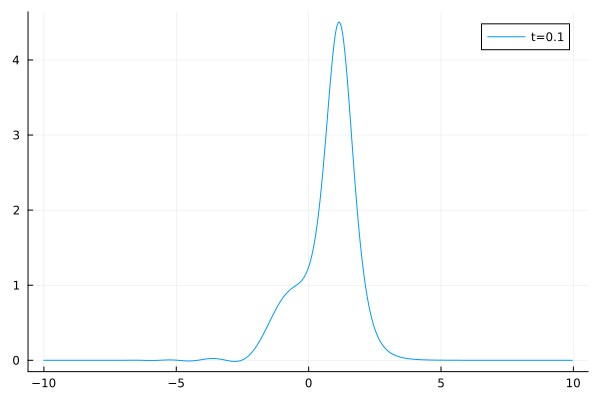
\includegraphics[width=\linewidth]{images/2-1.png}
                \caption{Solution at $t=0.1$.}
                \label{fig2:a}
                \vspace{4ex}
            \end{subfigure}%%
            \begin{subfigure}[b]{0.45\linewidth}
                \centering
                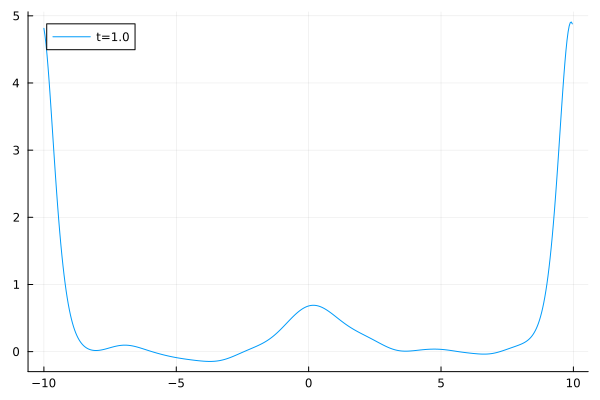
\includegraphics[width=\linewidth]{images/2-2.png}
                \caption{Solution at $t=1.0$.}
                \label{fig2:b}
                \vspace{4ex}
            \end{subfigure}
            \begin{subfigure}[b]{0.45\linewidth}
                \centering
                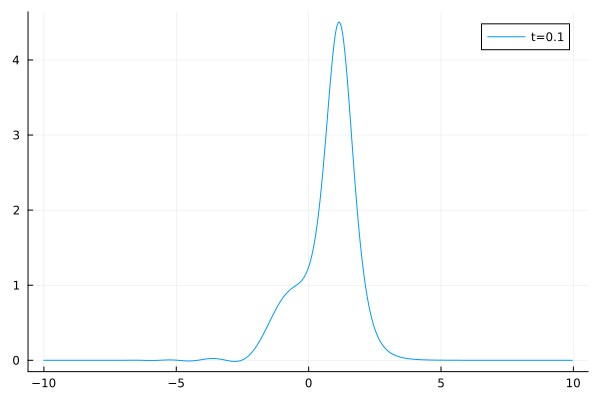
\includegraphics[width=\linewidth]{images/2-1.png}
                \caption{Solution at $t=2.0$.}
                \label{fig2:c}
                \vspace{4ex}
            \end{subfigure}%%
            \begin{subfigure}[b]{0.45\linewidth}
                \centering
                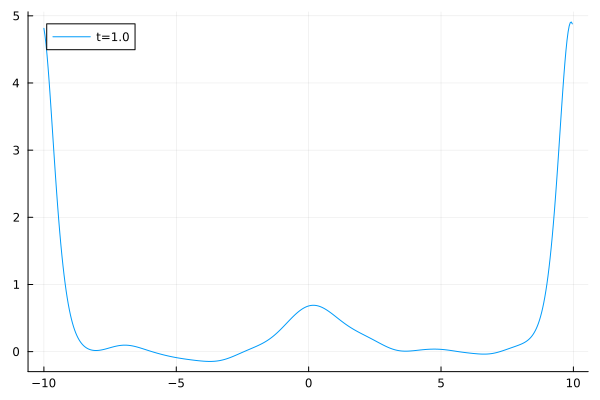
\includegraphics[width=\linewidth]{images/2-2.png}
                \caption{Solution at $t=4.0$.}
                \label{fig2:d}
                \vspace{4ex}
            \end{subfigure}
            \caption{Solutions at $t=[0.1,1.0,2.0,4.0]$ to the KdV equation using a second-order accurate method.}
            \label{fig2}
        \end{figure}


        \item [(b)]
        We hope that this second-order method is Lax-Richtmyer stable when studying the eigenvalues of the Jacobian used in Newton's method. Since we are time-stepping using the trapezoid rule, we will map the eigenvalues of the Jacobian using $z=k\lambda$ where $z \mapsto  \frac{1-z}{1+z}$. For the trapezoid method to be stable, we expect the eigenvalues to lay within the unit circle. To gain an understanding of the eigenvalues' behavior during the solving process, we compute, using Julia's \verb+eigvals+ function, and graph the eigenvalue of each Jacobian during Newton's method and apply the above mapping. We modified the Newton's method presented above as following
        \begin{python}
function Newton(U,U0,m,F,DF)
    count = 0
    New_U = U0
    update = fill(100,m+1)
    while maximum(abs.(update)) > 1e-10
        count += 1
        if count == 300
            @printf("No convergence")
        break
        end
        update = DF(New_U)\F(New_U,U)
        New_U = New_U - update
        #compute evals
        evals = eigvals(Df(New_U) |> Matrix)
        bur = z -> (1-z)/(1+z)
        lambdamap = bur.(k*evals)
        graph = plot!(real(lambdamap),imag(lambdamap),seriestype=:scatter,xaxis=[-1.1,1.1],legend=false)
    end
    return New_U
end
        \end{python}
        Running the same problem presented in the previous part for $t\in[0.15,0.30,0.6,1.20]$, we compute the eigenvalues of 60, 120, 242, and 489 Jacobians and plotting their values we see that the eigenvalues all lay along the unit circle and do not extend far outside, as seen in Figure \ref{fig2evals}. We thus expect this method to be Lax-Richtmyer stable due to the consistency of eigenvalues laying on and near the unit disk.
        
        \begin{figure}[H]
            \begin{subfigure}[b]{0.45\linewidth}
                \centering
                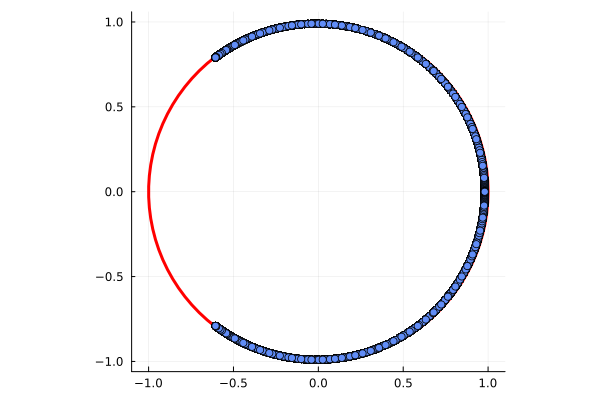
\includegraphics[width=\linewidth]{images/2b-1.png}
                \caption{Mapped eigenvalues of 60 Jacobains at $t=0.15$.}
                \label{fig2evals:a}
                \vspace{4ex}
            \end{subfigure}%%
            \begin{subfigure}[b]{0.45\linewidth}
                \centering
                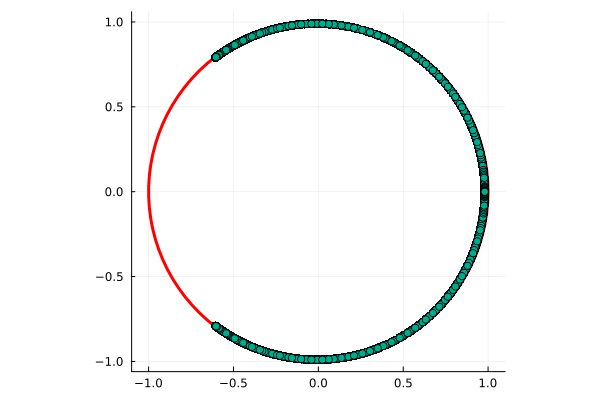
\includegraphics[width=\linewidth]{images/2b-2.png}
                \caption{Mapped eigenvalues of 120 Jacobains at $t=0.30$.}
                \label{fig2evals:b}
                \vspace{4ex}
            \end{subfigure}
            \begin{subfigure}[b]{0.45\linewidth}
                \centering
                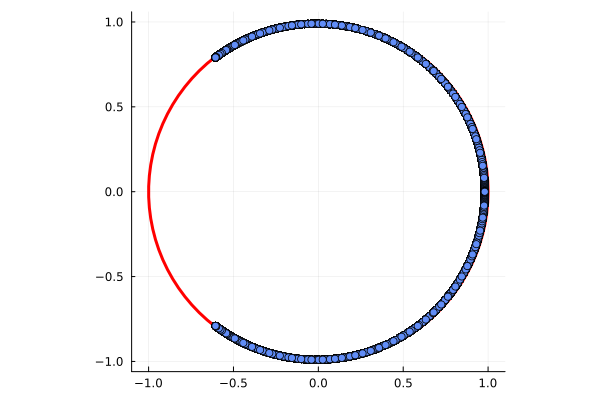
\includegraphics[width=\linewidth]{images/2b-1.png}
                \caption{Mapped eigenvalues of 242 Jacobains at $t=0.60$.}
                \label{fig2evals:c}
                \vspace{4ex}
            \end{subfigure}%%
            \begin{subfigure}[b]{0.45\linewidth}
                \centering
                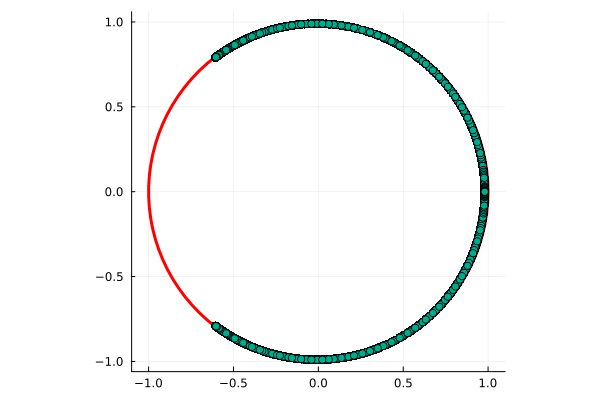
\includegraphics[width=\linewidth]{images/2b-2.png}
                \caption{Mapped eigenvalues of 489 Jacobains at $t=1.20$.}
                \label{fig2evals:d}
                \vspace{4ex}
            \end{subfigure}
            \caption{Mapped eigenvalues of Jacobian for solutions at $t\in[0.15,0.30,0.6,1.20]$ to the KdV equation using a second-order accurate method.}
            \label{fig2evals}
        \end{figure}


    \end{enumerate}
    


\end{solution}

%----------------------------------------------------------------------------------------------------%
%\vskip 20pt
\newpage

%---------------%
%---Problem 1---%
%---------------%

%--status--$

\begin{problem}
    Consider solving the small-dispersion (semi-classical) focusing NLS equation
    \begin{align*}
        \begin{cases}
            i \epsilon u_t + \frac{\epsilon^2}{2} u_{xx} + |u|^2 u = 0, \quad -\infty < x < \infty,\\
            u(x,0) = A(x) e^{i S(x)/\epsilon},\\
            A(x) = - \mathrm{sech}(x),\\
            S(x) = - \mu \log \cosh (x), \quad \mu = 0.1.
        \end{cases}
    \end{align*}
    Use the Fourier exponential integrator with Runge--Kutta 4 to solve this on $[-L, L]$ for sufficiently large $L$.  Use $\epsilon = 0.1$ and $\epsilon = 0.05$ and produce a contour plot of the squared modulus of the solution for $t \in [0,4]$ for both values of $\epsilon$.  Argue that you have chosen $L$ sufficiently large and have chosen a sufficiently large number of Fourier modes.
    
\end{problem}

\def\D{{\mathcal{D}}}
\def\c{{\check{c}}}
\newcommand{\mat}[1]{\begin{bmatrix}
    \\ #1 \\ \\
\end{bmatrix}}

\begin{solution}
    \noindent
    Consider solving the small-dispersion (semi-classical) focusing NLS equation
    \begin{align*}
        \begin{cases}
            i \epsilon u_t + \frac{\epsilon^2}{2} u_{xx} + |u|^2 u = 0, \quad -\infty < x < \infty,\\
            u(x,0) = A(x) e^{i S(x)/\epsilon},\\
            A(x) = - \mathrm{sech}(x),\\
            S(x) = - \mu \log \cosh (x), \quad \mu = 0.1.
        \end{cases}
    \end{align*}
    Rearranging the equation to get
    \[
        u_t = \frac{\epsilon i}{2} u_{xx} + \frac{i}{\eps}|u|^2 u,
    \]
    where $i$ denotes the imaginary unit. We wish to use the Fourier exponential integrator with RK4 to solve this on $[-L,L]$ for sufficiently large $L$. We begin by defining
    \[
        \F_N,\F_N^{-1},
    \] 
    to be the discrete Fourier transform and its inverse, tailored to the interval $[-L,L]$. That is, if
    \[
        f(x) = \frac{1}{\sqrt{2L}}\sum_{j=-N_{-}}^{N_{+}} \check{c}_j e^{i j \frac{\pi}{L}x},
    \]
    then
    \begin{align*}
        \F_N\paren{\mat{f(\check{x}_l)}} = \mat{c_j},\\
        \F^{-1}_N \paren{\mat{c_j}} = \mat{f(\check{x}_l)}, 
    \end{align*}
    where $\check{x}_l = -L + 2L \paren{\frac{l-1}{N}}, l=1,2,\cdots,N$ and $N_+ = \lfloor \frac{N}{2} \rfloor$ and $N_- = \lfloor \frac{N-1}{2} \rfloor.$ We also define
    \[
        \mathcal{D}_N = \frac{i\pi}{L}\mathrm{diag}(-N_{-},-N_{-}+1,\cdots,N_{+}).
    \]
    Now we can discretize the nonlinear term $|u|^2u$ as
    \[
        \mathcal{A}\paren{\mat{\check{c}_j}} = \frac{i}{\eps}\F_N \paren{ \left| \F_n^{-1}\paren{\mat{\c_j}}\right|^2 \circ \F_n^{-1}\paren{\mat{\c_j}} },
    \]
    where $\circ$ denotes that Hadamard product. So, we rewrite the PDE as
    \[
        \mat{\c_j(t)'} = \frac{\eps i}{2}D_N^2\mat{\c_j} + \mathcal{A}\paren{\mat{\c_j}}. 
    \] 
    Now letting 
    \[
        \mat{v_j(t)} = e^{\frac{-\eps i}{2}D_N^2 t}\mat{\c_j},
    \]
    we get
    \[
        \mat{v_j(t)'} = e^{\frac{-\eps i}{2}D_N^2 t}\mathcal{A}\paren{e^{\frac{\eps i}{2}D_N^2 t} \mat{v_j(t)}}.
    \]
    Hoping that
    \[
        \mat{u(\check{x}_j,t)} \approx \F_N^{-1}\paren{\mat{\c_j(t)}},
    \]
    we employ RK4 as a time stepper. The method is implemented in Julia as follows:
    \begin{python}
mfftshift = x -> circshift(fftshift(x), isodd(length(x)) ? 1 : 0)
mfft = x -> fftshift(fft(fftshift(x),1)) # fft(x,1) is used so that
mifft = x -> mfftshift(ifft(mfftshift(x),1))
mgrid = (n,L) -> -L .+ 2*L*(0:n-1)/n
diffvec = (L,m,j) -> ((-floor(m/2):1:floor((m-1)/2))*(1im*pi/L)).^j

function rk4(F,k,t,c)
    f1 = k*F(c,t)
    f2 = k*F(c + .5*f1, t + .5*k)
    f3 = k*F(c + .5*f2, t + .5*k)
    f4 = k*F(c + f3, t + k)
    return c + 1/6.0*(f1 + 2.0*f2 + 2.0*f3 + f4)
end

function solve_shrody(eps,k,T,L,m)
    mu = 0.1
    S(x) = mu * log.(cosh.(x))
    A = x -> - sech.(x)
    eta = x -> A.(x).*exp.(1im*S.(x)/eps)

    X = mgrid(m,L)
    c = mfft(eta(X))
    U = mifft(c)
    cl = [-2,2]

    d2 = (eps* 1im)/(2)*diffvec(L,m,2)

    N = v -> (1im/eps)*v.*abs2.(v)

    F = (v,tau) -> exp.(-d2*tau).*(mfft(N(mifft(exp.(d2*tau).*v))))


    n = convert(Int64,ceil(T/k))

    ts = 0:k:T
    z = zeros(size(X)[1],n+1)

    for i = 2:n+1
        c = exp.(d2*k).*rk4(F,k,0.0,c)
        U = mifft(c)
        z[:,i] = abs2.(U)
    end 
    return ts,X,z
end
    \end{python}

    \noindent
    To find an $L$ that is sufficiently large for the method, we require the solution, note that throughout our work, 'solution' refers to the modulus squared of the approximate solution, to go to zero at the edges of the domain. Let's pick $L=25$ and using $h=0.001$ and $t\in[0,4]$, we compute the maximum value along the edges throughout time using the $z$ matrix the code generates. In Julia, we implement this as
    \begin{python}
z = solve_shrody(epsilon,0.001,4,25,m)[3]
max_l = maximum(z[1,:])
max_r = maximum(z[end,:])
    \end{python}    
    Running the code for $\eps = 0.1$ and $\eps=0.05$ we find that:
    \begin{center}
        \begin{tabular}{ c|c|c }
          & $\eps=0.1$ & $\eps=0.05$ \\ 
         \hline
         \verb+max_l+ & 3.28135217179093e-11 & 5.658338560671543e-7 \\  
         \verb+max_r+ & 2.4169893980594823e-11 & 2.971566893335267e-7    
        \end{tabular}
    \end{center}
    Therefore $L=25$ seems like a reasonable choice for both $\eps=0.1$ and $\eps=0.05$. On later thought, we notice that the boundary conditions are periodic and thus the computation of \verb+max_r+ is not needed.


    \noindent
    Next, we will find a sufficient number of Fourier modes $m$. Let's pick $m=2^{15}$. To check if this choice of $m$ is reasonable, we compute the solution with $L=25, h=0.001$, $t\in[0,4]$ and $m=2^{15}$ and $m/2$. Then comparing the maximum difference between the solutions using the following Julia code
    \begin{python}
z = solve_shrody(epsilon,0.001,4,2^15)
z_half = solve_shrody(epsilon,0.001,4,2^15/2)
dif = z_half - z[1:2:end,:]
maxdif = maximum(dif)
    \end{python}
    Running this method for $\eps=0.1$ and $\eps=0.05$ we get that the max difference is:
    \begin{center}
        \begin{tabular}{ c|c|c }
          & $\eps=0.1$ & $\eps=0.05$ \\ 
         \hline
         \verb+maxdif+ & 6.266898111562114e-11 & 4.624698917155001e-7
        \end{tabular}
    \end{center}
    Since the error between the solution with $m$ modes and $m/2$ modes is small, and thus we argue that our choice of $m$ is sufficiently large.

    \noindent
    Now that we have found sufficient $L$ and $m$ values, we compute the solution using $h=0.001, L=25,m=2^15,\and t\in[0,4]$ to get the contour plots presented in figure \ref{fig3}. We note that looking at the contour plots we once again see that that our choice of $L$ is sufficient.

    \begin{figure}[H]
        \begin{subfigure}[b]{0.5\linewidth}
            \centering
            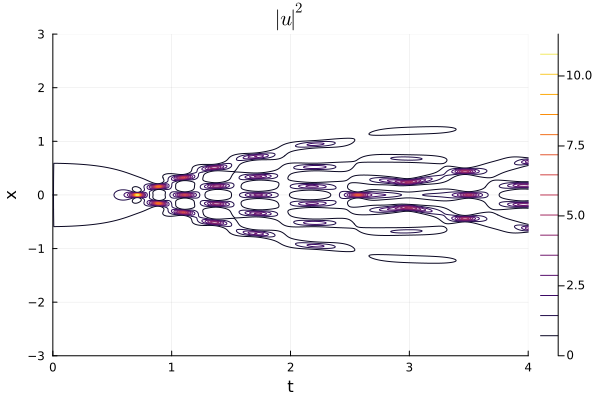
\includegraphics[width=\linewidth]{images/3-1.png}
            \caption{Contour when $\eps=0.1$.}
            \label{fig3:a}
            \vspace{4ex}
        \end{subfigure}%%
        \begin{subfigure}[b]{0.5\linewidth}
            \centering
            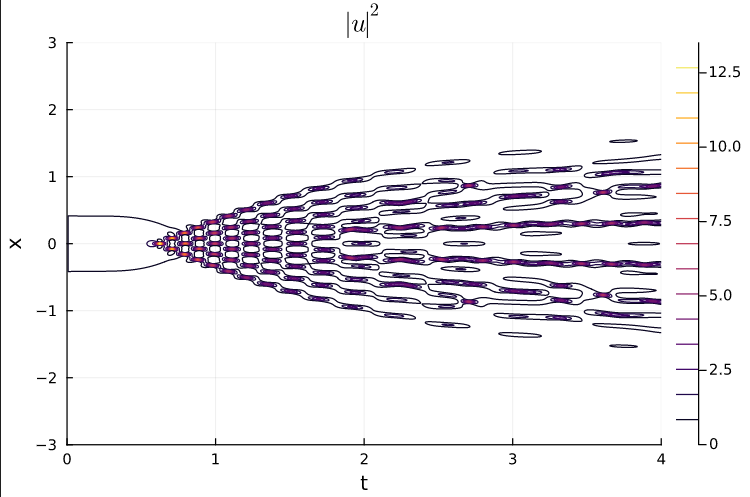
\includegraphics[width=\linewidth]{images/3-2.png}
            \caption{Contour when $\eps=0.05$.}
            \label{fig3:b}
            \vspace{4ex}
        \end{subfigure}
        \caption{Contour plot of the solution to focusing NLS using Fourier exponential using RK4 where $\eps=0.1$ and $\eps=0.05$.}
        \label{fig3}
    \end{figure}
\end{solution}

%----------------------------------------------------------------------------------------------------%
%\vskip 20pt
\newpage

%---------------%
%---Problem 1---%
%---------------%

%--status--$

\begin{problem}
    Consider solving the Kuramoto-Sivashinsky equation with periodic boundary conditions
 \begin{align*}
    \begin{cases} u_t + u u_x + u_{xx} + u_{xxxx} = 0, \quad -L < x <L,\\
      u(x,0) = \eta(x),\\
      u(-L,t) = u(L,t),\\
      u_x(-L,t) = u_x(L,t),\\
      u_{xx}(-L,t) = u_{xx}(L,t),\\
      u_{xxx}(-L,t) = u_{xxx}(L,t).
    \end{cases}
 \end{align*}
 Use the ETDRK4 method using Fourier series to solve this problem with $L = 16 \pi$, $\eta(x) = \cos(x/16) (1 + \sin(x/16))$.  Create a contour plot of the solution for $t \in [0,150]$.
\end{problem}

\begin{solution}
    
    \noindent
    Consider the Kuramoto-Sivashinsky equation with periodic boundary conditions
    \begin{align*}
        \begin{cases} u_t + u u_x + u_{xx} + u_{xxxx} = 0, \quad -L < x <L,\\
          u(x,0) = \eta(x),\\
          u(-L,t) = u(L,t),\\
          u_x(-L,t) = u_x(L,t),\\
          u_{xx}(-L,t) = u_{xx}(L,t),\\
          u_{xxx}(-L,t) = u_{xxx}(L,t).
        \end{cases}
     \end{align*}
     We will modify the given ETDRK4 method using Fourier series to solve this problem with $L=16\pi$, $\eta(x) = \cos(x/16)(1 + \sin(x/16))$. The modified code looks like
     \begin{python}
init = x ->  cos.(x ./ 16) .* (1 .+ sin.(x ./ 16))

L = 16 * pi
N = 2^10
X = mgrid(N,L)
c = mfft(init(X))
D1 = diffvec(L,N,1)
D2 = diffvec(L,N,2)
D4 = diffvec(L,N,4)
U = mifft(c)
cl = [-10,10]
k = 0.1

NF = c -> mfft(-mifft(c).*mifft(D1.*c))

S0 = Diagonal(exp.(-(D2+D4)*k/2))
S1 = Diagonal(exp.(-(D2+D4)*k))

E0 = k*stable_eval(f0, -(D2+D4)*k, 2) |> Diagonal
E1 = k*stable_eval(f1, -(D2+D4)*k, 2) |> Diagonal
E2 = k*stable_eval(f2, -(D2+D4)*k, 2) |> Diagonal
E3 = k*stable_eval(f3, -(D2+D4)*k, 2) |> Diagonal

ts = 0:k:150
z = zeros(size(X)[1],size(ts)[1])

for i = 2:1500
    aa = S0*c + E0*NF(c)
    bb = S0*c + E0*NF(aa)
    cc = S0*aa + E0*(2*NF(bb)-NF(c))
    c = S1*c + E1*NF(c) + E2*(NF(aa) + NF(bb)) + E3*NF(cc)
    z[:,i] = mifft(c) |> real
end

#create contour plot
contour(ts,X,z)
     \end{python}
     Then using the \verb+contour+ function we create the contour plot shown in Figure \ref{fig4} of the solutions for $t\in[0,150]$.
     
     \begin{figure}[H]
        \centering
        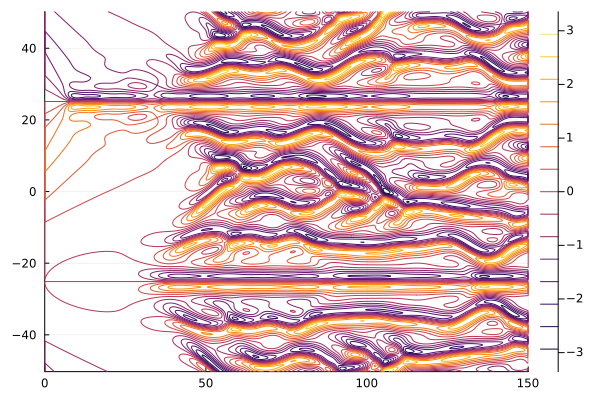
\includegraphics[width=0.75\textwidth,height=\textwidth,keepaspectratio]{images/4.png}
        \caption{Contour plot of solutions to the Kuramoto-Sivashinsky equation using ETDRK4 for $t\in[0,150]$.}
        \label{fig4}
     \end{figure}

\end{solution}

%----------------------------------------------------------------------------------------------------%
%\vskip 20pt
\end{document}